\section{Framework}
\label{framework}

CircuitModelPilot automates the iterative development of circuit predictors, from analyzing an existing model to implementing and evaluating a revised design. Given an AI4EDA task and an initial predictor, the framework uses LLM agents to inspect model behavior, identify potential deficiencies in the circuit-modeling formulation, and turn proposed improvements into executable candidates. Candidate designs are organized in a search tree so that the framework can explore alternatives, revisit earlier models, and use both positive and negative experimental feedback. The same workflow supports changes to circuit representations, neural computation, and learning objectives, together with training and hyperparameter optimization. This section formalizes the modeling problem, presents the overall architecture, and describes the components that implement this iterative search.

\subsection{Problem Formulation}
\label{sec:problem_formulation}

\subsubsection{Circuit Modeling as a Design Problem}

Let $\mathcal{D}_{\mathrm{tr}}$ and $\mathcal{D}_{\mathrm{val}}$ denote the training and validation data for an EDA prediction task. A modeling formulation is
\begin{equation}
    \mathcal{C}=(\phi,\psi,\ell),
    \label{eq:codesign_tuple}
\end{equation}
where $\phi$ constructs the circuit representation and its features, $\psi$ specifies the neural architecture and computation, and $\ell$ specifies the training objective, including any auxiliary supervision. These correspond to the representation, computation, and learning-signal dimensions discussed in Section~\ref{sec:semantic_codesign}. Training a candidate with configuration $\lambda$ produces parameters
\begin{equation}
    \theta=\operatorname{Train}(\mathcal{C},\lambda;
    \mathcal{D}_{\mathrm{tr}}),
    \label{eq:candidate_training}
\end{equation}
and a predictor $f_{\mathcal{C},\theta}(d)=\psi_{\theta}(\phi(d))$. We write its validation utility as
\begin{equation}
    q=Q(f_{\mathcal{C},\theta};\mathcal{D}_{\mathrm{val}}),
    \label{eq:validation_utility}
\end{equation}
with the metric direction normalized so that larger $q$ is better. For example, an error metric can be negated. The prediction target, label meaning, and validation metric remain fixed even when a candidate changes the objective used for gradient-based training. Thus, redesigning $\ell$ does not redefine what counts as a better predictor.

\subsubsection{Distinction from Fixed-Space NAS}

A conventional architecture-search formulation can be expressed as
\begin{equation}
    (a^\star,\lambda^\star)
    =\operatorname*{arg\,max}_{a\in\mathcal{A}_{\mathrm{NAS}},\,
    \lambda\in\Lambda} q(a,\lambda),
    \label{eq:fixed_nas}
\end{equation}
where $\mathcal{A}_{\mathrm{NAS}}$ and $\Lambda$ encode available architecture and training choices. Typically, circuit representation and supervision are supplied by the task designer; even when they are searchable, their alternatives must be expressible in the predefined space. Feedback guides selection among these encoded choices.

CircuitModelPilot instead constructs new formulations during search. At iteration $t$, it selects a parent $p$ and generates a modeling proposal $P_{t+1}$ using the task context $\kappa$, circuit knowledge $\mathcal{K}$, the current search tree $\mathcal{T}_t$, and the parent's experimental evidence $E_p$:
\begin{equation}
\begin{aligned}
 P_{t+1}&=\pi_{\mathrm{LLM}}
 (\kappa,\mathcal{K},\mathcal{T}_t,E_p),\\
 \mathcal{C}_{t+1}&=\operatorname{Implement}
 (\mathcal{C}_p,P_{t+1}).
\end{aligned}
\label{eq:adaptive_modeling}
\end{equation}
The proposal may introduce a graph transformation, a propagation mechanism, or a training objective whose implementation was not listed initially. The task interface and editable modules constrain these changes, but do not enumerate all resulting models. The LLM uses both performance and diagnostic evidence to decide what to construct, while the fixed validation utility still determines how candidates are compared.

Under a total search budget $B$, the output is selected from the successfully evaluated candidates $\mathcal{V}_{\mathrm{ok}}$:
\begin{equation}
\begin{aligned}
 i^\star&=\operatorname*{arg\,max}_{i\in\mathcal{V}_{\mathrm{ok}}}q_i,\\
 \sum_{r\in\mathcal{R}}c_r&\leq B,
\end{aligned}
\label{eq:semantic_search}
\end{equation}
where $\mathcal{R}$ includes all attempted runs and $c_r$ is their cost under the declared budget measure. This is a budgeted search over generated candidates, without a claim of global optimality. Training and tuning costs, including unsuccessful attempts, must be included consistently in comparisons with automated baselines.

\subsection{Overall Architecture}
\label{sec:framework_overview}

Figure~\ref{fig:framework} shows the CircuitModelPilot workflow. A task interface supplies circuit knowledge, data access, the initial model, and training and evaluation entry points. The search controller selects a parent from the model-design tree. A modeling agent diagnoses its limitations and proposes a revision; a candidate builder implements the revision and checks that the code matches the proposal. The execution component trains the candidate, optionally tunes its hyperparameters, and collects validation results. A result analyst interprets the evidence and recommends how exploration should proceed. The candidate and its analysis are then added to the tree, closing the feedback loop.

\begin{figure*}[t]
    \centering
    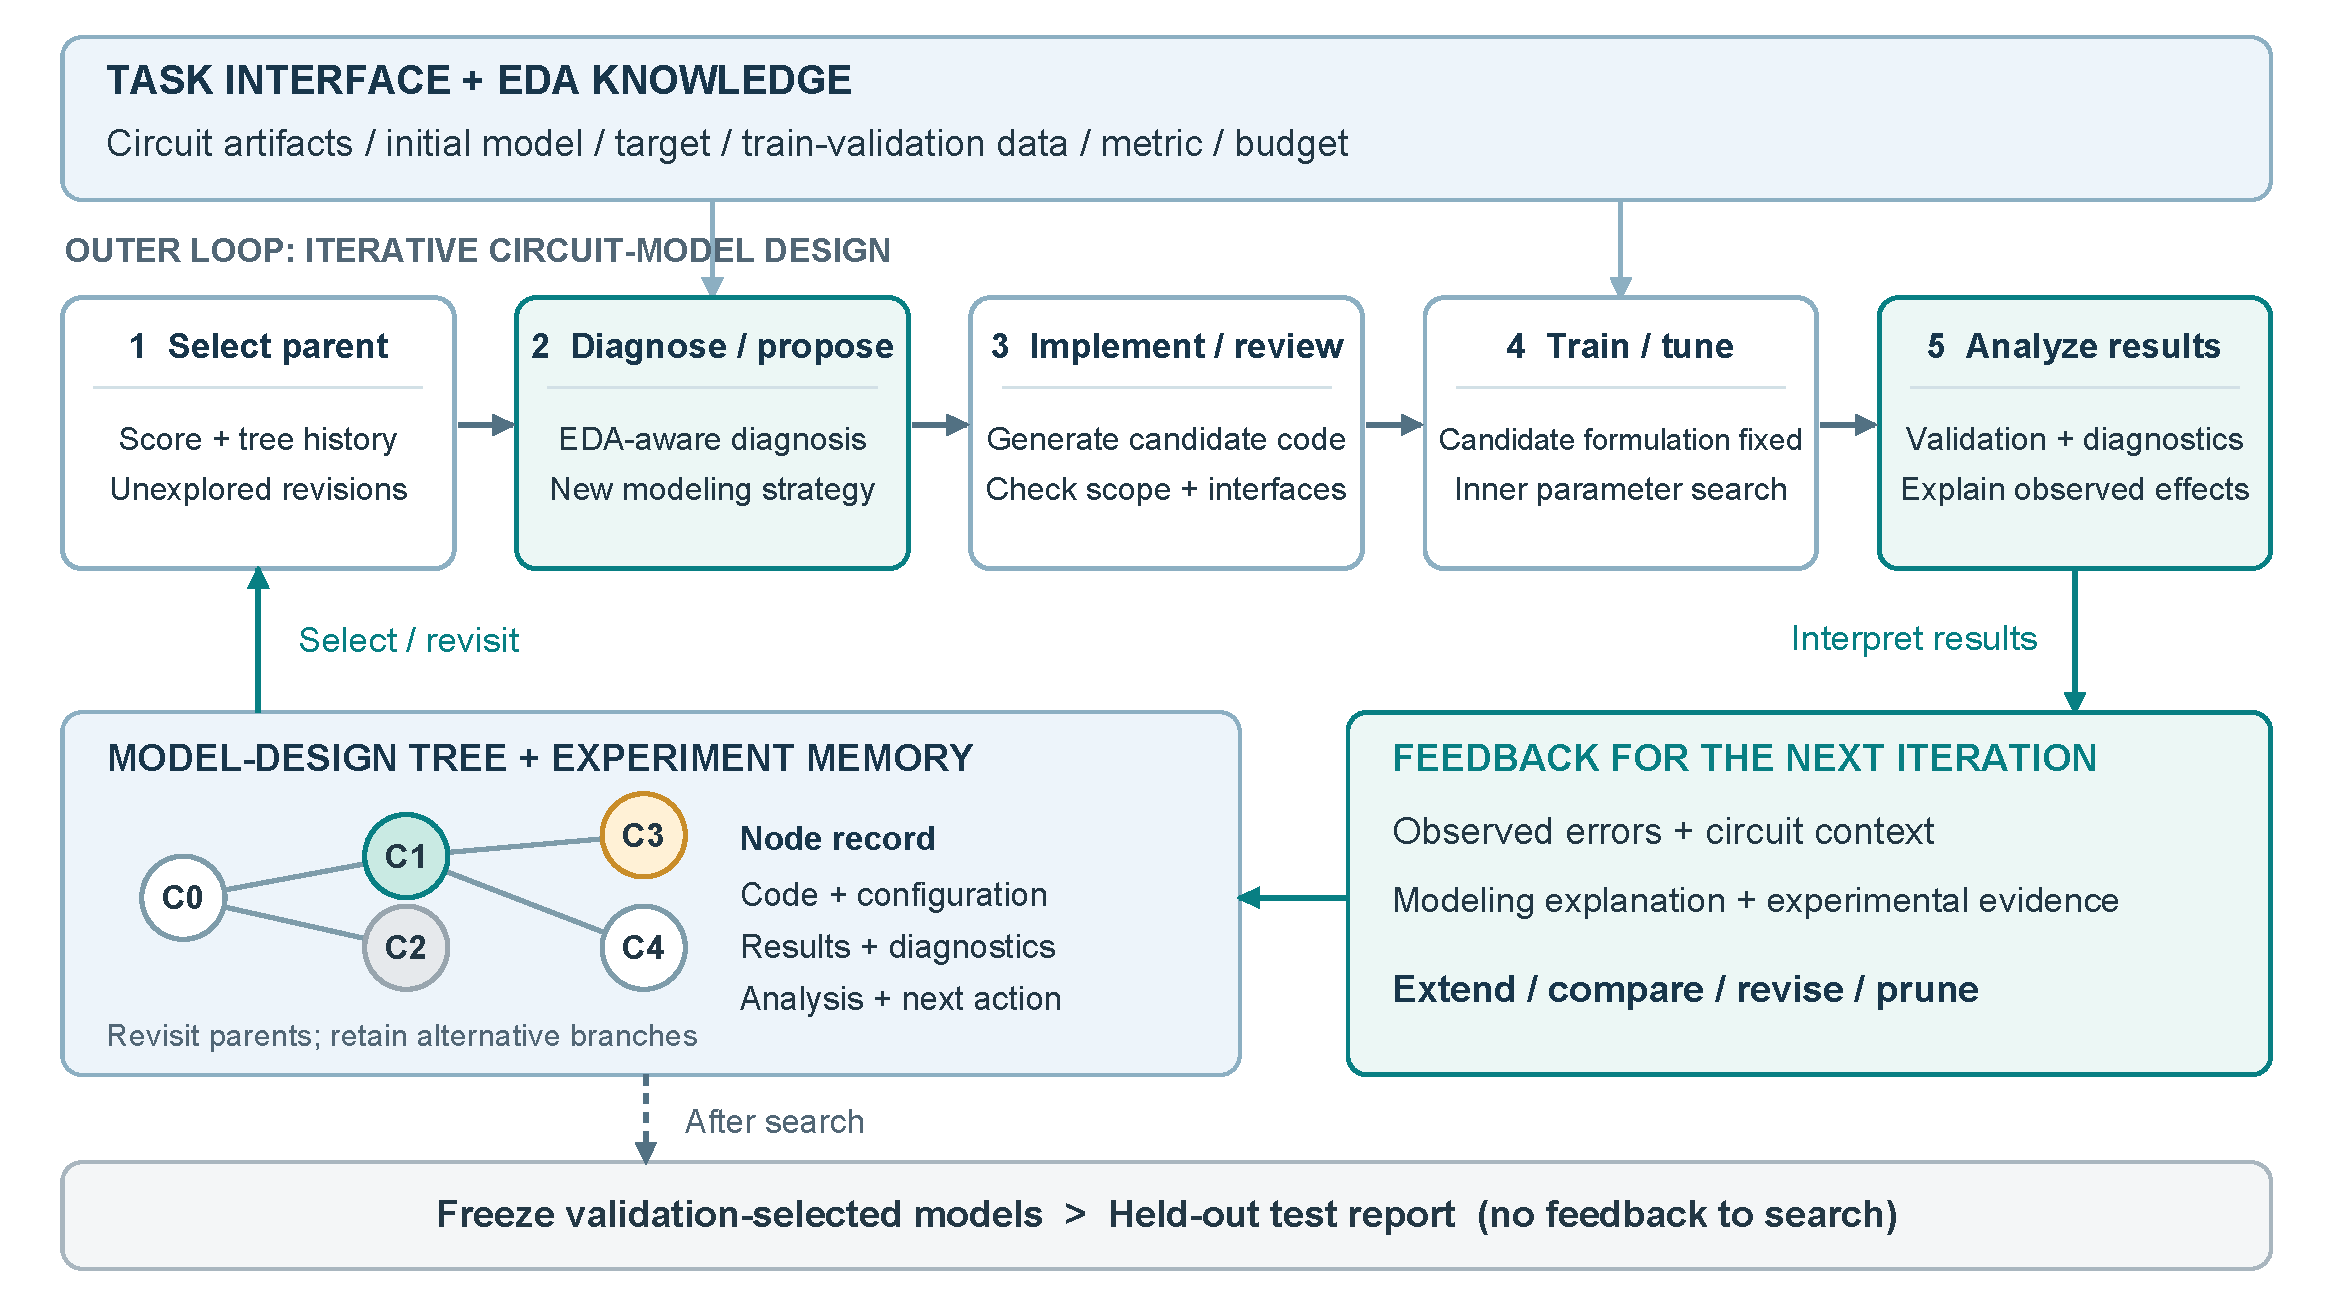
\includegraphics[width=\textwidth]{figs/CircuitModelPilot-framework.pdf}
    \caption{Overall architecture of CircuitModelPilot. The LLM-guided outer loop constructs and evaluates new circuit-modeling strategies, while the inner training and tuning stage optimizes each candidate. Circuit knowledge and validation diagnostics guide subsequent revisions through a persistent model-design tree. Held-out test evaluation occurs only after model selection and has no feedback path into search.}
    \label{fig:framework}
\end{figure*}

The components have distinct responsibilities: the modeling agent decides what to change, the builder realizes that change, the executor measures its effect, and the analyst determines what the evidence supports. They are roles in the workflow and need not correspond to different LLM families. Shared experiment records connect them across iterations and allow the search controller to return to an earlier candidate without reconstructing its state from a conversation history.

\subsection{Task Interface and EDA Knowledge}
\label{sec:task_interface}

Each task adapter defines the prediction target, available circuit artifacts, input and output contracts, initial predictor, permitted code modules, and training and validation procedures. It also fixes the data partition, metric definition, and budget policy in the task context $\kappa$. Candidate-generated preprocessing operates within this interface so that a representation change remains compatible with the task and does not alter the evaluation samples or their labels.

The adapter provides the domain information needed to interpret model behavior: circuit object and relation types, relevant analysis rules, feature meanings, and available diagnostic quantities. For netlist timing, this may include cell types, timing arcs, and path dependencies. For HLS prediction, it may include operations, data dependencies, and synthesis-related attributes. CircuitModelPilot uses this information together with model code and experimental observations to reason about what the current predictor captures and what it may omit. The framework therefore reuses a common agent workflow across tasks while retaining task-specific representations and diagnostics.

Domain knowledge also determines which questions can be answered by the available evidence. If a task exposes only aggregate error, the agent may request an additional validation diagnostic before proposing a structural change. It should not infer a particular circuit-level failure from the aggregate score alone. All diagnostics used for search are derived from the training or validation partition; the held-out test set remains outside the agent's working context.

\subsection{Model Diagnosis and Revision Proposals}
\label{sec:hypothesis_protocol}

For a selected parent, the modeling agent examines three sources of evidence: the current implementation, its validation and training behavior, and the history of related candidates. It relates observed errors to the task's circuit representation and analysis structure. For example, errors concentrated on deep timing paths may suggest insufficient propagation of delay information; errors concentrated on a cell category may suggest that distinct cell behavior is being aggregated too uniformly. These are possible explanations to investigate, rather than conclusions implied by an error pattern.

The agent converts its analysis into a concise modeling proposal containing the observed limitation, the proposed change, its implementation scope, and the diagnostic effect expected if the change is useful. The proposal is stored in the existing hypothesis-card artifact, but its purpose is practical: to connect a modeling decision to code and an experiment. A proposal can involve coordinated changes, such as adding a graph relation and its corresponding update rule, while unrelated changes are assigned to separate candidates so their effects remain interpretable.

The available revision dimensions are those in $\mathcal{C}$. Representation changes can expose additional circuit objects, features, or relations. Computation changes can revise message passing, aggregation, update order, or prediction heads. Learning changes can revise loss transformations or auxiliary supervision. The agent selects among these dimensions according to the observed limitation; it does not have to modify every dimension in each iteration. Prior failed attempts constrain later proposals by recording which modifications were tested and under what conditions they were unsuccessful.

\subsection{Candidate Implementation, Training, and Tuning}
\label{sec:scoped_realization}

\subsubsection{Code Generation and Candidate Review}

The builder copies the selected parent's generated modules into a candidate workspace and implements the proposed revision there. The supported modules include graph transformations, model and convolution definitions, and task-approved training components. The parent implementation is retained so that alternative children can branch from the same starting point.

Before training, a separate Candidate Review checks whether the proposed modeling change is realized in the code and whether additional changes have been introduced. Runtime checks validate interfaces, editable scope, and the task context. A failed implementation is repaired within the same proposal or recorded as an unsuccessful attempt. A code error is not treated as evidence that the modeling idea itself is ineffective. The candidate record retains the proposal, source snapshot, parent-relative changes, and execution configuration.

\subsubsection{Training and Inner Parameter Search}

For a fixed formulation $\mathcal{C}_i$, the executor trains the model and selects checkpoints using validation evidence. When enabled by the task, a separate inner search selects a training configuration:
\begin{equation}
 \lambda_i^\star=\operatorname*{arg\,max}_{\lambda\in\Lambda_i}
 Q\big(f_{\mathcal{C}_i,\theta_i(\lambda)};
 \mathcal{D}_{\mathrm{val}}\big),
 \label{eq:param_search}
\end{equation}
where $\Lambda_i$ is the declared set of permitted hyperparameters and $\theta_i(\lambda)$ is obtained by training under that configuration. In practice, this denotes the best evaluated configuration within the allocated tuning budget. The existing execution workflow uses Optuna for this stage when parameter search is requested.

This separation distinguishes a change in modeling formulation from a change in its optimization settings. Both may improve prediction, but their contributions are recorded separately. The executor returns the validation score, permitted error breakdowns, training statistics, execution status, and cost. These observations support both candidate ranking and the next round of modeling analysis.

\subsection{Tree-Structured Model Search}
\label{sec:trace_guided_exploration}
\label{sec:design_trace}

\subsubsection{Tree State and Parent Selection}

The search state is a rooted tree $\mathcal{T}_t=(\mathcal{V}_t,\mathcal{E}_t)$ initialized with the baseline model. Each node stores a candidate record
\begin{equation}
 T_i=(p_i,\mathcal{C}_i,P_i,\lambda_i,E_i,A_i),
 \label{eq:design_trace}
\end{equation}
where $p_i$ identifies the parent, $P_i$ is the proposal, $E_i$ contains execution and validation evidence, and $A_i$ records the analysis and suggested next action. An edge $(p_i,i)$ represents the implemented revision. Nodes retain their artifacts and execution status even when a branch is no longer expanded.

Let $\mathcal{F}_t$ denote the set of evaluated candidates eligible for further development. It can include an earlier internal node, not only the most recent leaves. Parent selection is expressed as
\begin{equation}
 p_t=\pi_{\mathrm{select}}
 (\mathcal{F}_t,\mathcal{T}_t,\kappa,\mathcal{K}).
 \label{eq:parent_selection}
\end{equation}
The controller uses the LLM to weigh validation performance, remaining modeling limitations, evidence from previous children, and the remaining budget. It can refine a strong candidate or revisit an earlier node when another modeling direction remains plausible. The selected parent and the rationale for expanding it are recorded with the next proposal.

\subsubsection{Expansion, Comparison, and Pruning}

Expanding a node creates a child with one coherent modeling revision. Siblings provide alternative responses to the same parent limitation, while deeper descendants accumulate useful changes. An ablation is represented as another child that removes or alters a component to investigate its effect. Re-evaluations can be recorded as children with unchanged model code to distinguish repeatability evidence from a newly designed model.

After evaluation, the controller updates the eligible set using the result analysis. A promising child can remain active for refinement; a branch with repeated negative evidence can be marked inactive; an ambiguous result can trigger a focused diagnostic or another run within budget. Pruning changes future search allocation without deleting the candidate or its evidence. Returning to the root or another earlier node creates an alternative path through the same tree. These operations preserve useful work while preventing the search from being tied to one sequence of edits.

Algorithm~\ref{alg:hedge_loop} summarizes the process. Every attempted execution contributes to the search record and consumes budget according to the declared policy. The search stops when the budget is exhausted, no eligible direction remains, or the controller records an explicit stop decision. No monotonic improvement is assumed: failed candidates are part of the evidence used to choose later revisions.

\begin{algorithm}[t]
\caption{Iterative Circuit-Model Search}
\label{alg:hedge_loop}
\begin{algorithmic}[1]
\REQUIRE Task context $\kappa$, knowledge $\mathcal{K}$, initial model $\mathcal{C}_0$, budget $B$
\STATE Evaluate $\mathcal{C}_0$; initialize tree $\mathcal{T}$ and eligible set $\mathcal{F}$
\WHILE{budget remains and $\mathcal{F}\neq\emptyset$}
    \STATE Select parent $p$ using performance and recorded analysis
    \STATE Diagnose $\mathcal{C}_p$; propose a modeling revision $P_i$
    \STATE Implement and review candidate $\mathcal{C}_i$
    \IF{candidate passes review and runtime checks}
        \STATE Train and optionally tune within remaining budget
        \STATE Collect validation results and permitted diagnostics
        \STATE Analyze the outcome and recommend a next action
    \ELSE
        \STATE Record implementation failure and repair feedback
    \ENDIF
    \STATE Store child record in $\mathcal{T}$; account for consumed budget
    \STATE Update eligible parents $\mathcal{F}$ and search memory
    \IF{controller records a stop decision}
        \STATE \textbf{break}
    \ENDIF
\ENDWHILE
\STATE Freeze validation-selected candidates for final reporting
\end{algorithmic}
\end{algorithm}

\subsection{Feedback-Driven Iteration and Final Selection}
\label{sec:feedback_iteration}

The result analyst converts each completed experiment into feedback for the next design decision. It first checks whether the intended change was executed and the comparison is valid. For a successfully evaluated child, its utility difference from the parent is
\begin{equation}
    \Delta q_i=q_i-q_{p_i}.
    \label{eq:parent_improvement}
\end{equation}
The analyst interprets this difference alongside circuit-specific error breakdowns, learning curves, and the parent-relative code changes. It separates an observed performance change from an explanation of that change: a better aggregate score alone does not establish that the proposed mechanism resolved the diagnosed limitation.

Feedback addresses three questions: what improved or degraded, what the evidence suggests about the current modeling formulation, and which experiment should follow. If the expected diagnostic behavior improves with the score, the next iteration can extend the candidate or test the contribution of its components. If an intended effect is absent, the agent can revise the explanation and return to an earlier model. If the outcome is unstable or the diagnostic evidence is insufficient, the next action can be a repeat or a narrower test. The existing analysis records express these outcomes as supported, refuted, or inconclusive, with actions such as extend, ablate, prune, restart, or stop.

For example, a timing candidate that changes message propagation can be evaluated both on aggregate validation error and on errors grouped by path depth. Improvement concentrated on deeper paths would provide more specific feedback than the aggregate score alone. If errors instead persist for particular cell types, the next proposal may investigate cell-dependent transformations. This illustrates how the framework uses circuit knowledge to move from an observed limitation to a modeling change, then uses the experiment to refine the next question.

Each analysis is saved with the corresponding node so that subsequent agents can inspect successful mechanisms, rejected alternatives, and unresolved questions. The tree supplies the candidate history; the feedback supplies the reasons for choosing the next branch. Together, they implement an iterative model-development strategy whose available revisions can expand as the LLM generates new code.

At the end of search, candidates are ranked using validation evidence only. Following the evaluation protocol in Section~\ref{sec:evaluation_protocol}, the top three successfully evaluated candidates, or all available candidates if fewer than three exist, are frozen for held-out reporting. Test results do not trigger additional revisions or re-ranking. The output includes the selected model implementations, training configurations, and experiment records needed to reproduce them.
